\documentclass[11pt,a4paper]{article}

\usepackage[T1]{fontenc}
\usepackage[utf8]{inputenc}
\usepackage[french]{babel}
\usepackage{amsmath,amssymb}
\usepackage[margin=2.3cm]{geometry}
\usepackage{booktabs}
\usepackage{array}
\usepackage{textcomp}
\usepackage{enumitem}
\usepackage{float}
\usepackage{graphicx}
\usepackage{caption}
\usepackage{upquote}
\usepackage[colorlinks=true,linkcolor=blue,citecolor=blue,urlcolor=blue]{hyperref}

\newsavebox{\implbox}
\newenvironment{implication}%
  {\par\medskip\begin{lrbox}{\implbox}\begin{minipage}{0.95\textwidth}%
   \textbf{Ce qu'il faut en retenir.}\itshape\ }%
  {\end{minipage}\end{lrbox}\noindent\fbox{\usebox{\implbox}}\par\medskip}

\newcommand{\ee}{\mathrm{e}}
\newcommand{\jj}{\mathrm{j}}

\title{\bfseries Explication du slide 8\\[1mm]
       \large « De la pente de phase à la distance »\\[2mm]
       \normalsize notes de lecture de \texttt{slides\_principe\_VNA.pdf}}
\author{Notes de travail --- projet LiteVNA}
\date{\today}

\begin{document}
\maketitle

\begin{abstract}
\noindent
Le slide 8 établit la formule qui relie la \emph{pente de la phase} à la
\emph{distance}, et énonce les trois conditions sous lesquelles la distance
mesurée est la bonne. Ces notes le reprennent terme à terme, montrent sur des
courbes calculées ce que fait chaque terme, et appliquent le résultat à la
mesure du 17 septembre 2026, où une plaque métallique placée à $30$, $40$, $50$
puis $60$~cm donne un écart moyen de $36{,}5$~cm qui n'est pas tout à fait
constant.
\end{abstract}

\tableofcontents
\bigskip\hrule\bigskip

%=======================================================================
\section{Ce que dit le slide}
%=======================================================================

Après la correction SOL, le retour d'une cible isolée s'écrit
\[
  S_{11,\text{cible}}(f) = \alpha\,\ee^{\jj\theta(f)}\,
  \ee^{-\jj 4\pi f d / c},
\]
où $d$ est la distance de la cible et $\theta(f)$ une \emph{phase
supplémentaire}, c'est-à-dire tout ce qui s'ajoute après le plan de
calibration. Pour $\alpha > 0$, la phase déroulée et le retard estimé valent
\[
  \phi(f) = \theta(f) - \frac{4\pi f d}{c},
  \qquad
  \tau_{\text{mes}} = -\frac{1}{2\pi}\frac{\mathrm{d}\phi}{\mathrm{d}f}
  = \frac{2d}{c} - \frac{1}{2\pi}\frac{\mathrm{d}\theta}{\mathrm{d}f},
  \qquad
  \hat d = \frac{c\,\tau_{\text{mes}}}{2}.
\]

En mots :

\begin{enumerate}[label=\textbf{\arabic*.}]
\item \textbf{Le trajet dans l'air produit une phase qui décroît linéairement
      avec la fréquence.} Le facteur $4$ vient de l'aller-retour : la phase
      accumulée vaut $-2\pi f \times (2d/c)$.
\item \textbf{La pente de cette droite est le retard.} Mesurer une distance,
      c'est donc mesurer une pente, et non chercher la position d'un maximum.
\item \textbf{Toute phase supplémentaire s'ajoute à la pente par sa dérivée.}
      Si $\theta$ est elle-même un retard, elle décale la distance mesurée
      d'une quantité constante.
\end{enumerate}

\paragraph{Pourquoi la condition $\alpha > 0$.}
Si $\alpha$ était négatif --- par exemple la réflexion sur une plaque
métallique, où $\Gamma = -1$ --- la phase déroulée porterait un $\pi$
supplémentaire. Cela ne change pas la pente, donc pas la distance, mais cela
décale la constante et peut faire dérailler l'algorithme de déroulement.

%=======================================================================
\section{Un retard, c'est une droite}
%=======================================================================

\begin{figure}[H]
\centering
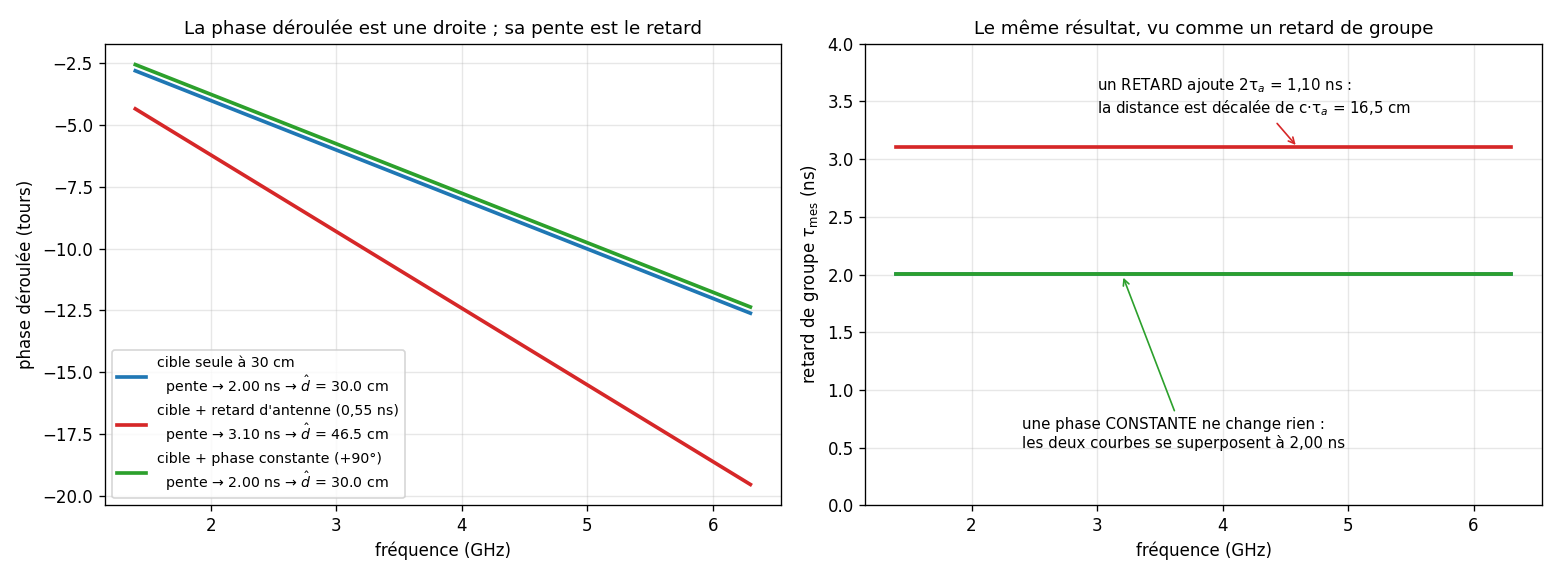
\includegraphics[width=\textwidth]{fig_pente_phase.png}
\caption{Phase déroulée et retard de groupe pour une cible à $30$~cm, calculés
sur $1{,}4$--$6{,}3$~GHz. \textbf{Une phase constante ne change pas la pente},
donc pas la distance : les courbes bleue et verte se superposent. Un
\textbf{retard} d'antenne de $0{,}55$~ns ajoute $2\tau_a = 1{,}10$~ns à la
pente, et décale la distance de $c\,\tau_a = 16{,}5$~cm.}
\label{fig:pente}
\end{figure}

La figure~\ref{fig:pente} illustre les deux cas élémentaires. Elle donne la
règle de conversion la plus utile de tout ce document :

\begin{implication}
Si la phase supplémentaire est un retard pur $\tau_a$ \emph{aller simple}, alors
$\hat d = d + c\,\tau_a$. \textbf{Le décalage affiché est le retard aller simple
de l'antenne, exprimé en distance dans l'air.} Un retard de $1$~ns se lit comme
$30$~cm.
\end{implication}

\paragraph{Une condition pratique au déroulement de phase.}
Entre deux points de fréquence, la phase ne doit pas tourner de plus d'un
demi-tour, sans quoi le déroulement est ambigu :
\[
  \Delta f < \frac{c}{4\,d_{\max}}.
\]
Pour une cible à $1$~m, cela fait $75$~MHz. Un balayage de $201$ points sur
$1{,}4$--$6{,}3$~GHz donne $24{,}5$~MHz : la marge est confortable.

%=======================================================================
\section{Ce que contient $\theta(f)$}
%=======================================================================

La correction SOL place l'origine des distances là où les étalons ont été
vissés. $\theta(f)$ rassemble donc tout ce qui se trouve \emph{après} ce plan :

\begin{itemize}
\item le trajet interne de l'antenne, du connecteur jusqu'à la zone qui
      rayonne ;
\item un adaptateur ou un bout de câble resté en aval du plan de calibration ;
\item le déplacement du centre de phase de l'antenne avec la fréquence ;
\item la réponse propre de la cible, si elle n'est pas un simple miroir.
\end{itemize}

Pour une ligne de longueur physique $L$ et de permittivité effective
$\varepsilon_{\text{eff}}$, le retard vaut $L\sqrt{\varepsilon_{\text{eff}}}/c$,
donc le décalage affiché vaut simplement $L\sqrt{\varepsilon_{\text{eff}}}$ :

\begin{table}[H]
\centering
\begin{tabular}{lcccc}
\toprule
Longueur $L$ & microstrip FR4 & coplanaire FR4 & tout dans le FR4 & air \\
 & ($\varepsilon_{\text{eff}} = 3{,}1$) & ($2{,}7$) & ($4{,}4$) & ($1$) \\
\midrule
$30$~mm  & $5{,}3$~cm & $4{,}9$~cm & $6{,}3$~cm & $3{,}0$~cm \\
$50$~mm  & $8{,}8$~cm & $8{,}2$~cm & $10{,}5$~cm & $5{,}0$~cm \\
$80$~mm  & $14{,}1$~cm & $13{,}1$~cm & $16{,}8$~cm & $8{,}0$~cm \\
$120$~mm & $21{,}1$~cm & $19{,}7$~cm & $25{,}2$~cm & $12{,}0$~cm \\
\bottomrule
\end{tabular}
\caption{Décalage affiché produit par une ligne de transmission, selon le
milieu. Un coaxial PTFE ($\varepsilon_r = 2{,}1$) affiche $1{,}45\,L$.}
\label{tab:lignes}
\end{table}

%=======================================================================
\section{Les trois conditions du slide}
%=======================================================================

La dernière phrase du slide énonce trois conditions. Voici ce qu'elles
signifient, et où en est notre banc.

\begin{table}[H]
\centering
\begin{tabular}{>{\raggedright\arraybackslash}p{4.0cm}
                >{\raggedright\arraybackslash}p{5.6cm}
                >{\raggedright\arraybackslash}p{5.4cm}}
\toprule
Condition & Ce qu'elle veut dire & État au 17/09/2026 \\
\midrule
« la phase supplémentaire est \textbf{constante} »
  & $\mathrm{d}\theta/\mathrm{d}f = 0$ : aucun biais de distance
  & Non : l'écart mesuré vaut $36{,}5$~cm \\
\addlinespace
« \textbf{ou corrigée} »
  & on mesure le biais une fois et on le retranche
  & C'est le rôle de \texttt{calibration.py -{}-plan} \\
\addlinespace
« le retour de la cible est \textbf{isolé} »
  & un seul écho dans la fenêtre d'analyse
  & Non : la structure fixe vers $20$~cm dépasse de $10$~dB l'écho de la
    plaque, et les lobes font $20$~cm de large \\
\bottomrule
\end{tabular}
\caption{Les trois conditions, appliquées à la mesure sur plaque métallique.}
\label{tab:conditions}
\end{table}

La troisième est la plus traîtresse. Quand deux échos se recouvrent, la phase
mesurée est celle de \emph{leur somme} : sa pente est une moyenne pondérée des
deux retards, et cette moyenne se déplace dès que les amplitudes relatives
changent --- donc dès que la cible s'éloigne.

%=======================================================================
\section{Quand $\theta$ dépend de la fréquence}
%=======================================================================

\begin{figure}[H]
\centering
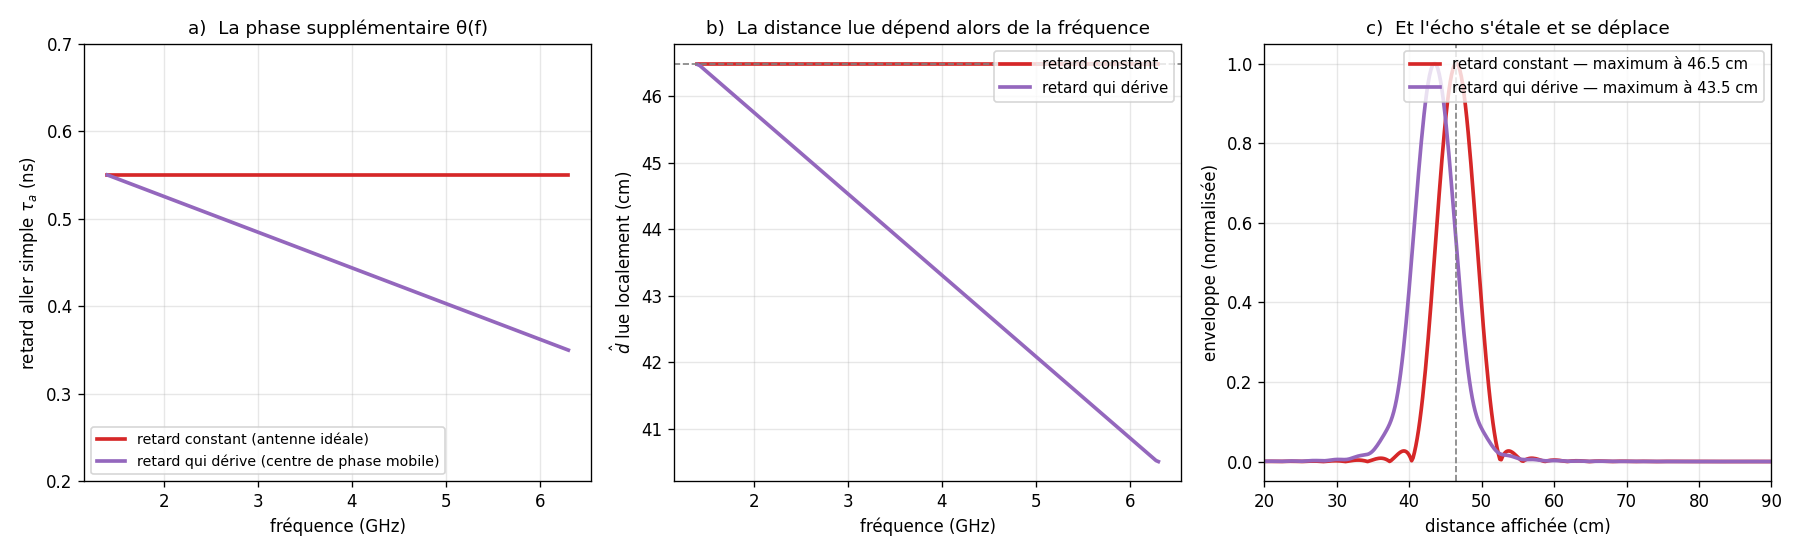
\includegraphics[width=\textwidth]{fig_dispersion.png}
\caption{Effet d'une phase supplémentaire dispersive. À gauche, le retard aller
simple de l'antenne : constant (rouge) ou dérivant de $0{,}55$ à $0{,}35$~ns
(violet), ce que produit un centre de phase qui se déplace. Au centre, la
distance lue localement : elle n'est plus unique. À droite, le profil de
distance : l'écho s'étale et son maximum se déplace de $46{,}5$ à
$43{,}5$~cm.}
\label{fig:dispersion}
\end{figure}

Deux mécanismes rendent $\theta$ dépendante de la fréquence :

\begin{description}[style=nextline, leftmargin=1.2em]
\item[Le centre de phase se déplace] Sur une antenne planaire large bande, la
  distribution de courant n'occupe pas la même zone à $1{,}4$ et à
  $6{,}3$~GHz. Le point d'où part l'onde se déplace, donc le retard change.
\item[Le substrat est dispersif] La permittivité du FR4 passe d'environ $4{,}4$
  à $1$~GHz à $4{,}2$ à $6$~GHz. Une ligne de $50$~mm voit alors son décalage
  varier de $1{,}4$~mm sur la bande, soit $4{,}8$~ps.
\end{description}

Ces variations ne déplacent pas seulement l'écho : \textbf{elles l'étalent},
puisque chaque fréquence arrive avec son propre retard. C'est une explication
possible des lobes de $20$~cm de large observés, là où la résolution
$c/2B$ n'en prévoit que $3$.

%=======================================================================
\section{Conséquence : la distance lue dépend de la bande}
%=======================================================================

\begin{figure}[H]
\centering
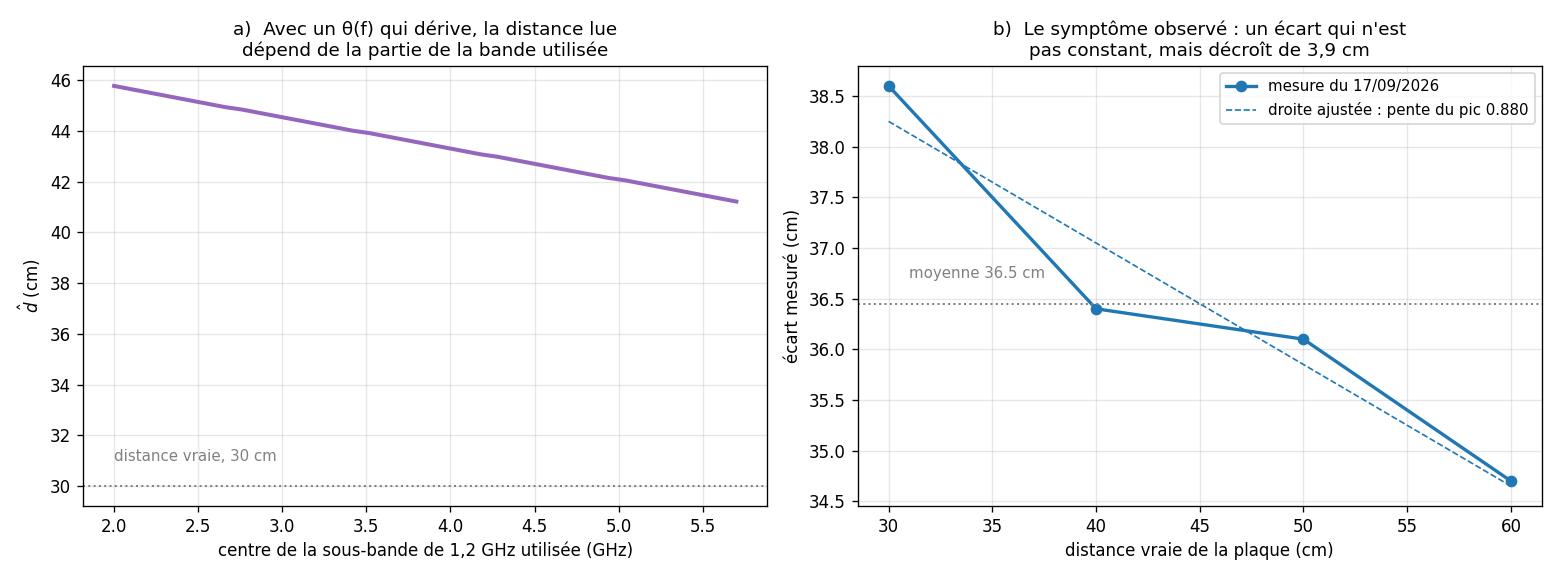
\includegraphics[width=\textwidth]{fig_bande.png}
\caption{À gauche, simulation : avec le $\theta(f)$ dispersif de la
figure~\ref{fig:dispersion}, la distance lue sur une sous-bande de
$1{,}2$~GHz varie de $4{,}6$~cm selon l'endroit de la bande choisi. À droite,
la mesure du 17/09 : l'écart décroît de $3{,}9$~cm quand la plaque s'éloigne de
$30$ à $60$~cm.}
\label{fig:bande}
\end{figure}

C'est le point qui relie la théorie du slide à l'observation. Si $\theta$ est
dispersive, la distance mesurée dépend de la partie de la bande qui domine
l'écho. Or cette pondération change avec la distance, pour au moins deux
raisons :

\begin{itemize}
\item \textbf{la plaque tronque le bas de la bande quand elle s'éloigne.} Elle
  ne se comporte en miroir que si elle couvre la première zone de Fresnel, de
  rayon $\sqrt{\lambda d/2}$, qui grandit avec la distance et avec la longueur
  d'onde ;
\item \textbf{les échos parasites ne décroissent pas comme celui de la cible},
  donc leur poids relatif change.
\end{itemize}

L'ordre de grandeur concorde : $4{,}6$~cm en simulation, $3{,}9$~cm mesurés.

%=======================================================================
\section{Deux contrôles numériques}
%=======================================================================

\paragraph{La période de la phase.}
Un écart de $36{,}45$~cm correspond à $\tau_a = 1{,}216$~ns aller simple, donc
à $2{,}43$~ns aller-retour. Une phase qui tourne à ce rythme fait un tour
complet tous les $411$~MHz :

\begin{table}[H]
\centering
\begin{tabular}{lcc}
\toprule
Mesure & Retard aller-retour & Période de la phase \\
\midrule
antenne seule, rien devant & $2{,}43$~ns & $411$~MHz \\
plaque à $30$~cm & $4{,}43$~ns & $226$~MHz \\
plaque à $60$~cm & $6{,}43$~ns & $156$~MHz \\
\bottomrule
\end{tabular}
\caption{Ce qu'on doit voir sur la phase de $S_{11}$ si le décalage est bien un
retard.}
\label{tab:periodes}
\end{table}

\paragraph{La borne géométrique.}
L'antenne employée est une biconique planaire de $120 \times 120$~mm. D'après le
tableau~\ref{tab:lignes}, même en faisant parcourir à l'onde tout le côté de la
carte dans le FR4, le décalage ne peut pas dépasser $25$~cm, et la valeur
réaliste est de $5$ à $13$~cm. Les $36{,}5$~cm mesurés demandent donc une
explication supplémentaire : un reste de câble en aval du plan de calibration,
ou une correction SOL non appliquée au traitement.

%=======================================================================
\section{Ce que le projet en fait}
%=======================================================================

\begin{itemize}
\item \texttt{calibration.py -{}-plan D1 D2} mesure le décalage avec une plaque
  à deux distances connues : c'est la « correction » de la deuxième condition.
  Il vérifie que la \textbf{pente} vaut $1$ et refuse d'écrire au-delà de
  $5\,\%$ d'écart --- une pente différente de $1$ signale justement que
  $\theta$ n'est pas un simple retard.
\item \texttt{qualification.py -{}-centre-phase} mesure $\theta(f)$ : c'est la
  seule façon de séparer un retard constant d'une dispersion.
\item Le budget du projet est serré. Pour tenir $0{,}1$~mm sur l'épaisseur du
  cartilage, il faut $0{,}65$~mm sur l'axe des distances, soit un retard de
  groupe stable à $\pm 2{,}2$~ps sur toute la bande.
\end{itemize}

\begin{implication}
La recette qui découle du slide : mesurer la \textbf{pente de phase} plutôt que
la position d'un maximum ; vérifier que cette pente est la même sur toute la
bande ; et ne retenir une valeur de plan d'antenne que si elle l'est.
\end{implication}

%=======================================================================
\section*{Annexe --- reproduire les figures}
\addcontentsline{toc}{section}{Annexe --- reproduire les figures}
%=======================================================================

Les trois figures sont calculées par \texttt{figures\_explication\_slide\_8.py},
dans ce dossier, qui réutilise \texttt{profil\_distance} du projet : la fenêtre
et l'axe des distances sont donc exactement ceux des programmes de mesure.
\begin{quote}
\texttt{python figures\_explication\_slide\_8.py}\\
\texttt{pdflatex explication\_slide\_8\_de\_slides\_principe\_VNA.tex}
\end{quote}

\end{document}
